\subsubsection{Anemômetro Ultrassônico}
  
  Para compor o sistema de monitoramento das turbinas e a avaliação da produção de energia, sentiu-se a necessidade de utilizar
  o anemômetro. O anemômetro é um sensor que possibilita medir a velocidade e a direção em que o ar se desloca. Há vários tipos
  de anemômetros no mercado, com diferentes métodos de medição, precisão e manutenção. Entre os anemômetros comerciais, o tipo
  ultrassónico é o que possui maior precisão, confiabilidade nos valores medidos em qualquer tipo de ambiente, rápida resposta
  e maior tempo de manutenção em comparação aos outros tipos no mercado \cite{pereira07}.
  
  O anemômetro ultrassônico possibilita a medição da velocidade do vento , por meio da velocidade do som no ar. Possui usualmente
  sensores ultrassônicos dispostos em formato de tetraedro, com um sensor piezolétrico em cada extremidade \cite{ribeiro06}.
  Primeiramente para inicializar o processo de medição, o anemômetro produz um sinal de referência, que é enviado ao 
  transdutor-transmissor, logo depois que este recebe o sinal, emite-se um sinal ultrassônico, que no decorrer do caminho até 
  chegar ao transdutor-receptor, sofre interferências da velocidade causadas pelo deslocamento do vento. Quando o sinal finalmente
  chega ao transdutor receptor o sinal é processado e há a alteração do sinal de referência que é quantificado \cite{pereira07}.
  
  Dentre os modelos disponíveis no mercado escolheu-se o anemômetro ultrassônico Young Modelo 86000.
  Este modelo além de ser compacto, possui baixo consumo, marcação CE e um bom custo-benefício.
  
  O modelo 86000 custa em torno de \$1390,00 com os impostos sobre seu preço integral e de frete, seu custo em reais
  é em torno de R\$ 7.579,50.
  
  \begin{figure}[!htbp]
    \centering
    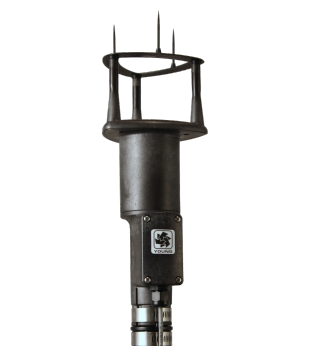
\includegraphics[scale=0.5]{editaveis/figuras/anemometro}
    \caption[Anemômetro ultrassônico Modelo 86000]
    {Figura ilustrativas do Anemômetro ultrassônico Modelo 86000 \footnotemark .}
    \label{anemometro}
  \end{figure}
  \footnotetext{Fonte: R.M. YOUNG COMPANY - OPERATING INSTRUCTIONS Model 86000 Ultrasonic Anemometer.}
  
  Abaixo as especificações técnicas do modelo 86000:
  
  \begin{figure}[!htbp]
    \centering
    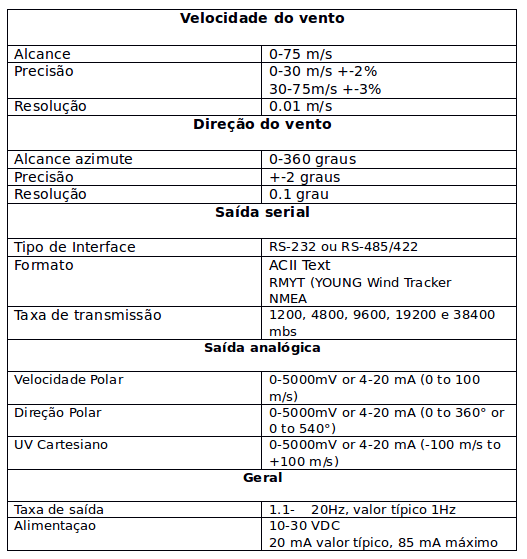
\includegraphics[scale=0.5]{editaveis/figuras/anemometro_spec}
    \caption[Especificações técnicas do anemômetro Modelo 86000]
    {Especificações técnicas do anemômetro Modelo 86000 \footnotemark .}
    \label{anemometro_spec}
  \end{figure}
  \footnotetext{Fonte: R.M. YOUNG COMPANY - OPERATING INSTRUCTIONS Model 86000 Ultrasonic Anemometer.}
  
  
  